
When setting up and especially when developing the system it is convenient to use the debug GUI seen in figure \ref{fig:debug GUI}. From here a lot of information can be obtained. 

In the upper left corner all cameras and their process steps can be seen. These can be selected and then poped to the grid, figure \ref{fig:grid}, by clicking \textit{Pop Window}. One a window configuration in the grid is set it can be saved by clicking \textit{Save grid configuration} under the Grid tab in the menu bar. 

In the upper right corner one can find profiling information for every step in the pipe line. In bottom of the window is the system log. This displays messages from inside the system. 

\begin{figure}[htb]
	\centering
	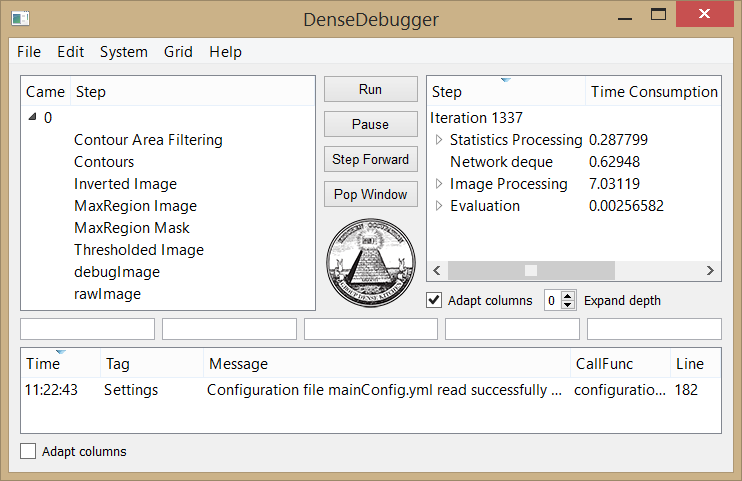
\includegraphics[width=\linewidth]{images/PosterDebugger.png}
	\caption[The debug GUI]
	{\textit{The debug GUI can be used by advanced users to get more detailed information about the system such as profiling and images of all the inherent process steps of the computer vision pipeline.}}
	\label{fig:debug GUI}  %Skapar referens till figuren
\end{figure}

\begin{figure}[htb]
	\centering
	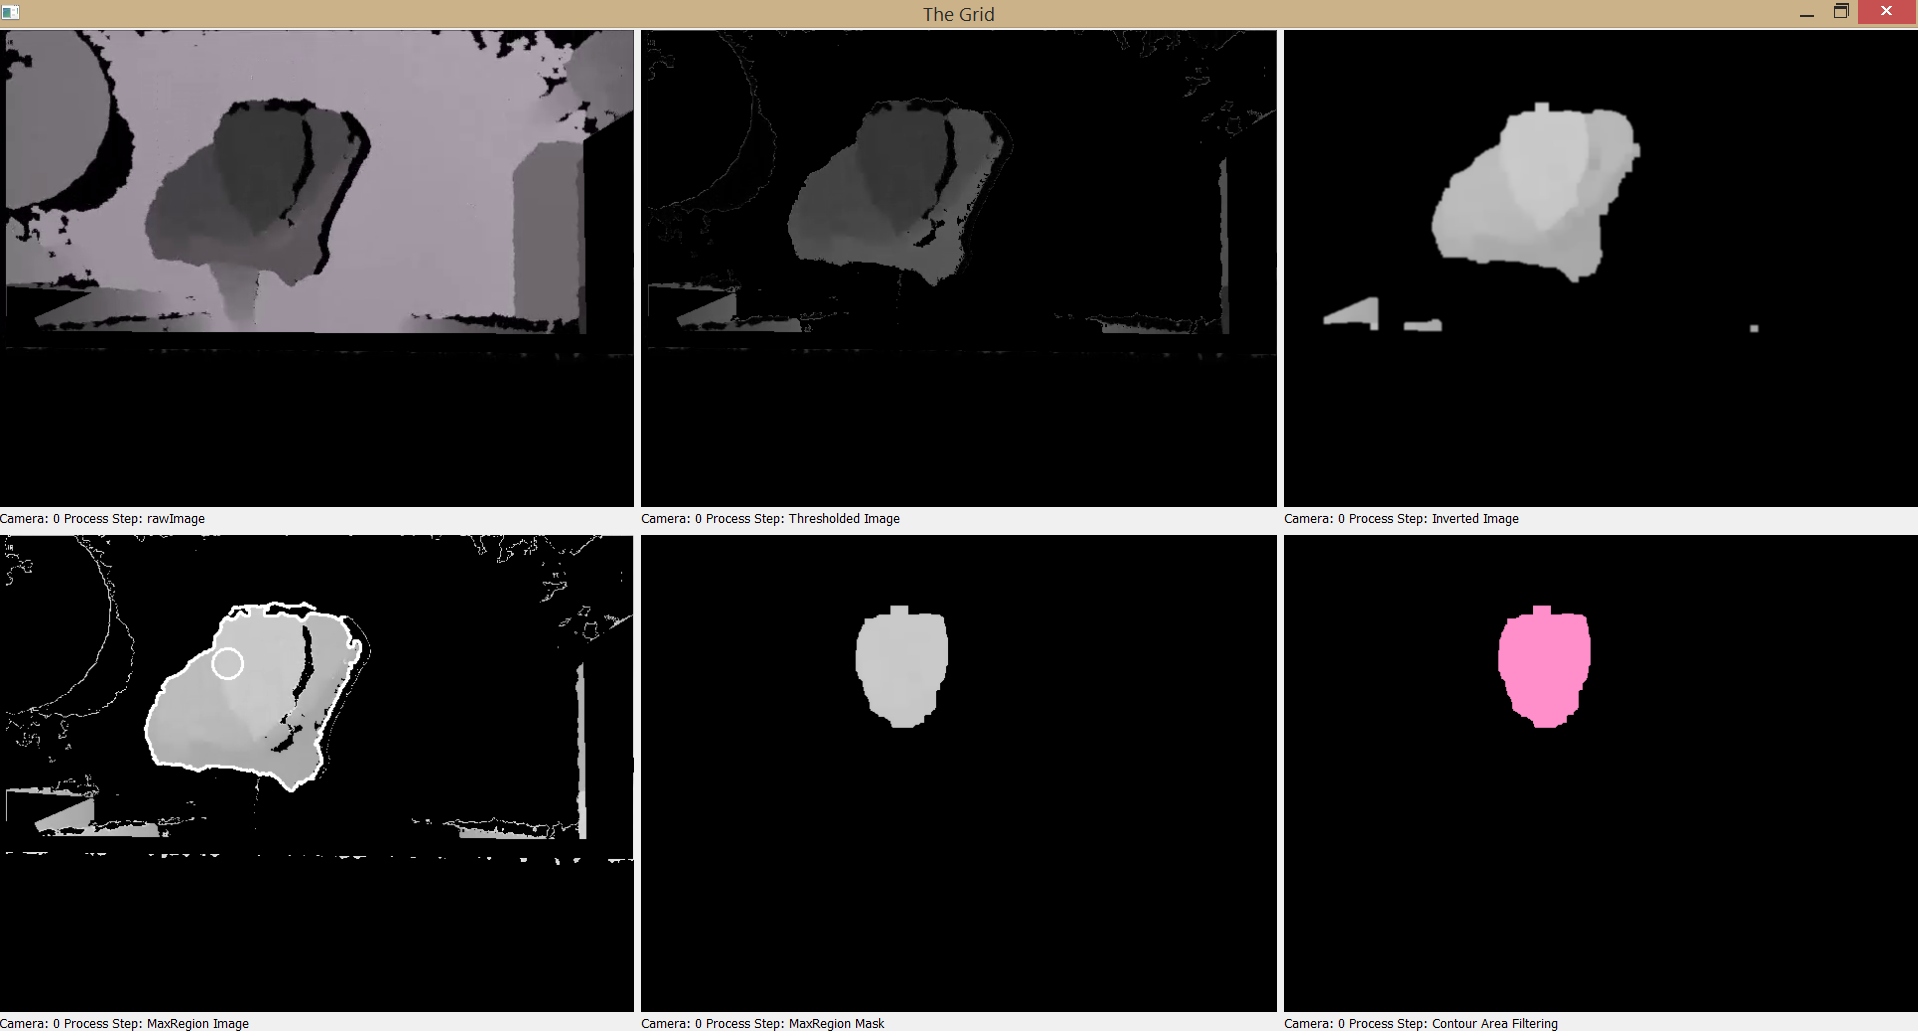
\includegraphics[width=\linewidth]{images/TheGrid.png}
	\caption[The grid]
	{\textit{The grid like a workspace to which you can send the process steps on which you are currently working. These can be stored to file to minimize manual window handling during development.}}
	\label{fig:grid}  %Skapar referens till figuren
\end{figure}
